\documentclass[tikz,border=2pt]{standalone}
\usepackage{pgfplots}
\pgfplotsset{compat=1.18}

\begin{document}
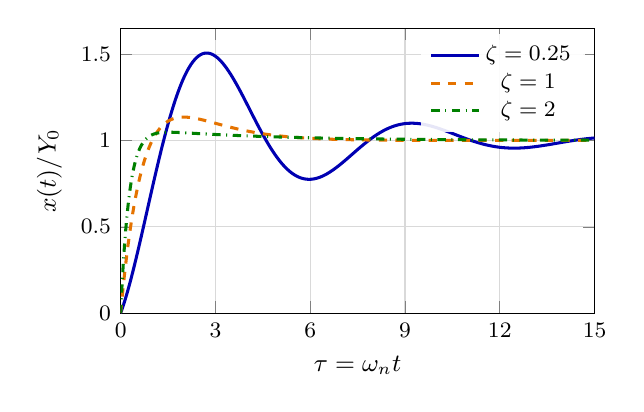
\begin{tikzpicture}
\begin{axis}[
    width=7.6cm,
    height=5.2cm,
    xmin=0,
    xmax=15,
    ymin=0,
    ymax=1.65,
    xlabel={$\tau=\omega_n t$},
    ylabel={$x(t)/Y_0$},
    xtick={0,3,6,9,12,15},
    ytick={0,0.5,1,1.5},
    grid=both,
    major grid style={draw=gray!30},
    tick label style={font=\footnotesize},
    label style={font=\small},
    legend style={
        at={(0.98,0.98)},
        anchor=north east,
        draw=none,
        fill=white,
        fill opacity=0.9,
        text opacity=1,
        font=\footnotesize,
        row sep=-1pt
    }
]
\addplot[
    blue!70!black,
    line width=1.1pt,
    domain=0:15,
    samples=500
] {1-exp(-0.25*x)*cos(deg(sqrt(1-0.25^2)*x))
    +(0.25/sqrt(1-0.25^2))*exp(-0.25*x)*sin(deg(sqrt(1-0.25^2)*x))};
\addlegendentry{$\zeta=0.25$}

\addplot[
    orange!90!black,
    dashed,
    line width=1.1pt,
    domain=0:15,
    samples=500
] {1+(x-1)*exp(-x)};
\addlegendentry{$\zeta=1$}

\addplot[
    green!50!black,
    dashdotted,
    line width=1.1pt,
    domain=0:15,
    samples=500
] {1+((-2-sqrt(3))*exp((-2-sqrt(3))*x)
    -(-2+sqrt(3))*exp((-2+sqrt(3))*x))/(2*sqrt(3))};
\addlegendentry{$\zeta=2$}
\end{axis}
\end{tikzpicture}
\end{document}
